% !TEX TS-program = pdflatex
% !TEX encoding = UTF-8 Unicode

% This is a simple template for a LaTeX document using the "article" class.
% See "book", "report", "letter" for other types of document.

\documentclass[11pt]{article} % use larger type; default would be 10pt

\usepackage[utf8]{inputenc} % set input encoding (not needed with XeLaTeX)

%%% Examples of Article customizations
% These packages are optional, depending whether you want the features they provide.
% See the LaTeX Companion or other references for full information.

%%% PAGE DIMENSIONS
\usepackage{geometry} % to change the page dimensions
\geometry{a4paper} % or letterpaper (US) or a5paper or....
% \geometry{margin=2in} % for example, change the margins to 2 inches all round
% \geometry{landscape} % set up the page for landscape
%   read geometry.pdf for detailed page layout information

\usepackage{graphicx} % support the \includegraphics command and options

% \usepackage[parfill]{parskip} % Activate to begin paragraphs with an empty line rather than an indent

%%% PACKAGES
\usepackage{booktabs} % for much better looking tables
\usepackage{array} % for better arrays (eg matrices) in maths
\usepackage{paralist} % very flexible & customisable lists (eg. enumerate/itemize, etc.)
\usepackage{verbatim} % adds environment for commenting out blocks of text & for better verbatim
\usepackage{subfig} % make it possible to include more than one captioned figure/table in a single float
% These packages are all incorporated in the memoir class to one degree or another...
\usepackage{amsmath}
\usepackage{amssymb}
\usepackage{graphicx}
\usepackage{float}
\usepackage{multirow}
%%% HEADERS & FOOTERS
\usepackage{fancyhdr} % This should be set AFTER setting up the page geometry
\pagestyle{fancy} % options: empty , plain , fancy
\renewcommand{\headrulewidth}{0pt} % customise the layout...
\lhead{}\chead{}\rhead{}
\lfoot{}\cfoot{\thepage}\rfoot{}

%%% SECTION TITLE APPEARANCE
\usepackage{sectsty}
\allsectionsfont{\sffamily\mdseries\upshape} % (See the fntguide.pdf for font help)
% (This matches ConTeXt defaults)

%%% ToC (table of contents) APPEARANCE
\usepackage[nottoc,notlof,notlot]{tocbibind} % Put the bibliography in the ToC
\usepackage[titles,subfigure]{tocloft} % Alter the style of the Table of Contents
\renewcommand{\cftsecfont}{\rmfamily\mdseries\upshape}
\renewcommand{\cftsecpagefont}{\rmfamily\mdseries\upshape} % No bold!

%%% END Article customizations

%%% The "real" document content comes below..
\title{}
\begin{document}
\maketitle
\section{Data}
The datasets used in the analysis were created by merging the students' responses data and the students' demographic data. The two datasets were merged using the unique deidentification code for each student (\textbf{deID}). The final analysis contains information on the following variables:

\begin{itemize}
\item Student Responses:
\begin{itemize}
\item \textbf{Confidence} (self-reported: three levels-- $0$ is low, $1$ is moderate and $2$ is high confidence)
\item \textbf{Self Evaluation} (self-reported: three levels-- ``different", ``close" or ``correct")
\item \textbf{Answer length} (derived: number of characters in the submitted answer)
\item \textbf{Criticism length} (derived: number of characters in the submitted criticism, typically submitted if the self evaltion is not ``correct")
\item \textbf{Submit Time} (recorded by the system (check this))
\item \textbf{Number of Questions} (derived: sum of the number of questions each student answered)
\end{itemize}
\item Student Characteristics:
\begin{itemize}
\item \textbf{Gender }
\item \textbf{Class Term} 
\item \textbf{Ethnicity }
\item \textbf{Proficiency Level} 
\item \textbf{Course Grade}
\item \textbf{UCLA Cumulative GPA}
\item \textbf{SAT Scores}
\item \textbf{High School GPA}
\item \textbf{Father's Education Level}
\item \textbf{Mother's Education Level} 
\end{itemize}

\item Recoded Variables

\begin{itemize}
\item \textbf{Numerical Self Eval} (``different'' $\rightarrow 0$, ``close" $\rightarrow 1$, ``correct" $\rightarrow 2$)
\item \textbf{PhD} (binary variable which takes value $1$ for a PhD student and $0$ otherwise, extracted from Proficiency Level; reference group is ``Undergraduate")
\item \textbf{MA} (binary variable which takes value $1$ for a MA student and $0$ otherwise, extracted from Proficiency Level; reference group is ``Undergraduate")
\item \textbf{Foreign} (binary variable which takes value $1$ for a foreign student and $0$ otherwise, extracted from Ethnicity; reference group is ``White")
\item \textbf{Asian} (binary variable which takes value $1$ for an asian student and $0$ otherwise, extracted from Ethnicity; reference group is ``White")
\item \textbf{Hispanic} (binary variable which takes value $1$ for a hispanic student and $0$ otherwise, extracted from Ethnicity; reference group is ``White")
\item \textbf{Female }(binary variable which takes value $1$ for a female student and $0$ otherwise, extracted from Gender)
\item \textbf{Term 11 }(binary variable which takes value $1$ for a Term 11 student and $0$ otherwise, extracted from Class Term; reference group is Term 15)
\item \textbf{Term 12 } (binary variable which takes value $1$ for a Term 12 student and $0$ otherwise, extracted from Class Term; reference group is Term 15)
\item \textbf{Term 13  }(binary variable which takes value $1$ for a Term 13 student and $0$ otherwise, extracted from Class Term; reference group is Term 15)
\end{itemize} 

\end{itemize}
\noindent
The merged dataset (from here on \textbf{Full Data}) was also used to create an aggregated dataset (from here on \textbf{Means Data}) by calculating mean numerical self evaluation and mean self confidence for each student. The Full Data consists of $6868$ observations, this is useful for more detailed analysis of effects but suffers from variable levels of representation of students (for eg: a student who submits only 2 responses is under-represented and another who submit 45 responses is over-respresented) . The Means Data consists of $212$ observations (corresponding to  $156$ unique male and  $56$ funique emale students), this leads to equal representation of each student but suffers from washing out some of the more subtle variation that can be tracked in the Full Data. 


\section{Analysis 1: Data Summary}
Some graphs and tables summarizing the data are presented next.

\subsection{Student Responses} 
First we note, that there doesn't appear to be any stastically significant differences in the answer lengths, criticism lengths and number of questions answered by male and female students. 
\begin{figure}[H]
\caption{Student responses by gender}
\centering
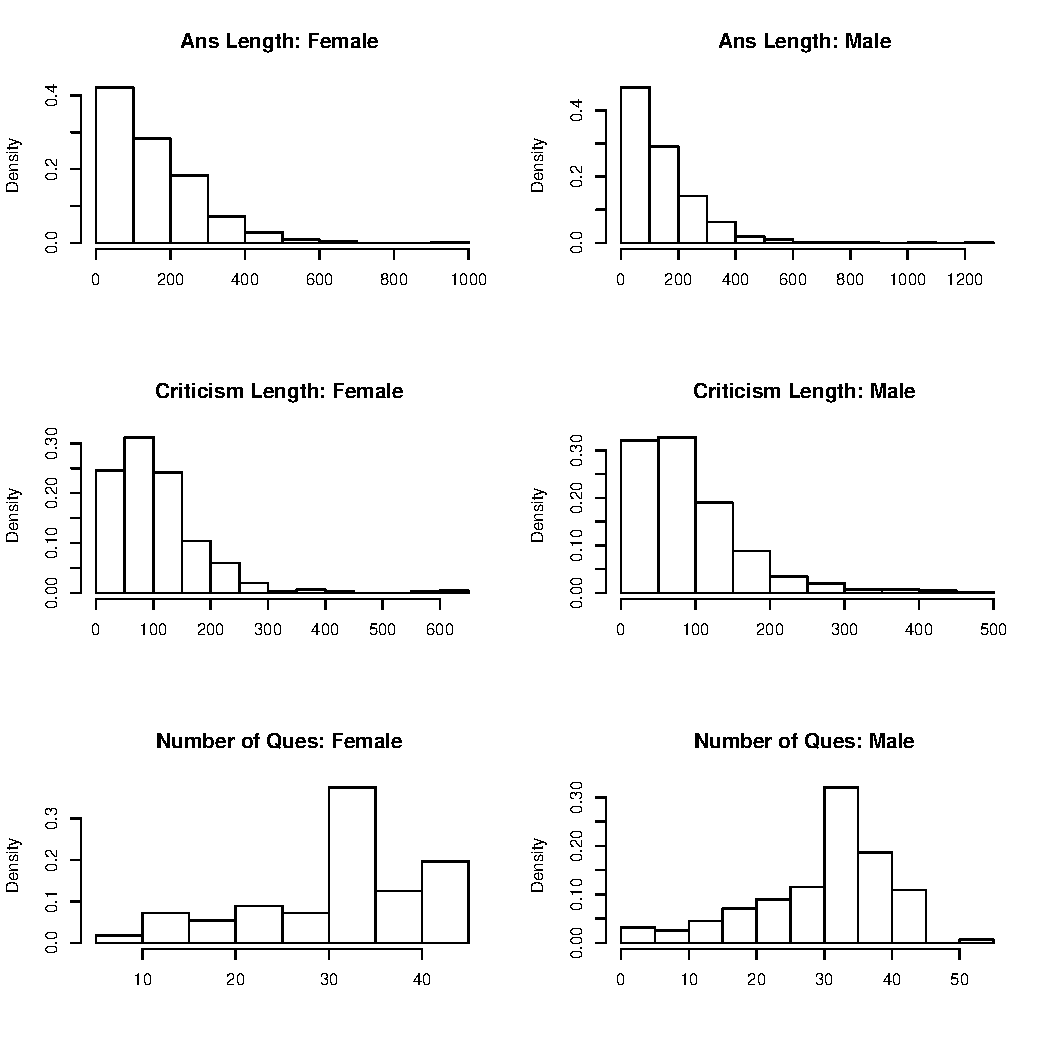
\includegraphics[width = 0.85 \textwidth]{comparison1.pdf}
\end{figure}
\newpage

\noindent
Since the main purpose of this analysis is the impact of confidence on student performance and participation, we now look at some statistics on confidence and self evaluation. At first glance, the distribution of confidence levels and self evaluation levels appear to be very similar across both genders, as implied by the following graphs. 
\begin{figure}[H]
\caption{Distribution of Confidence and Self Evaluation by gender}
\centering
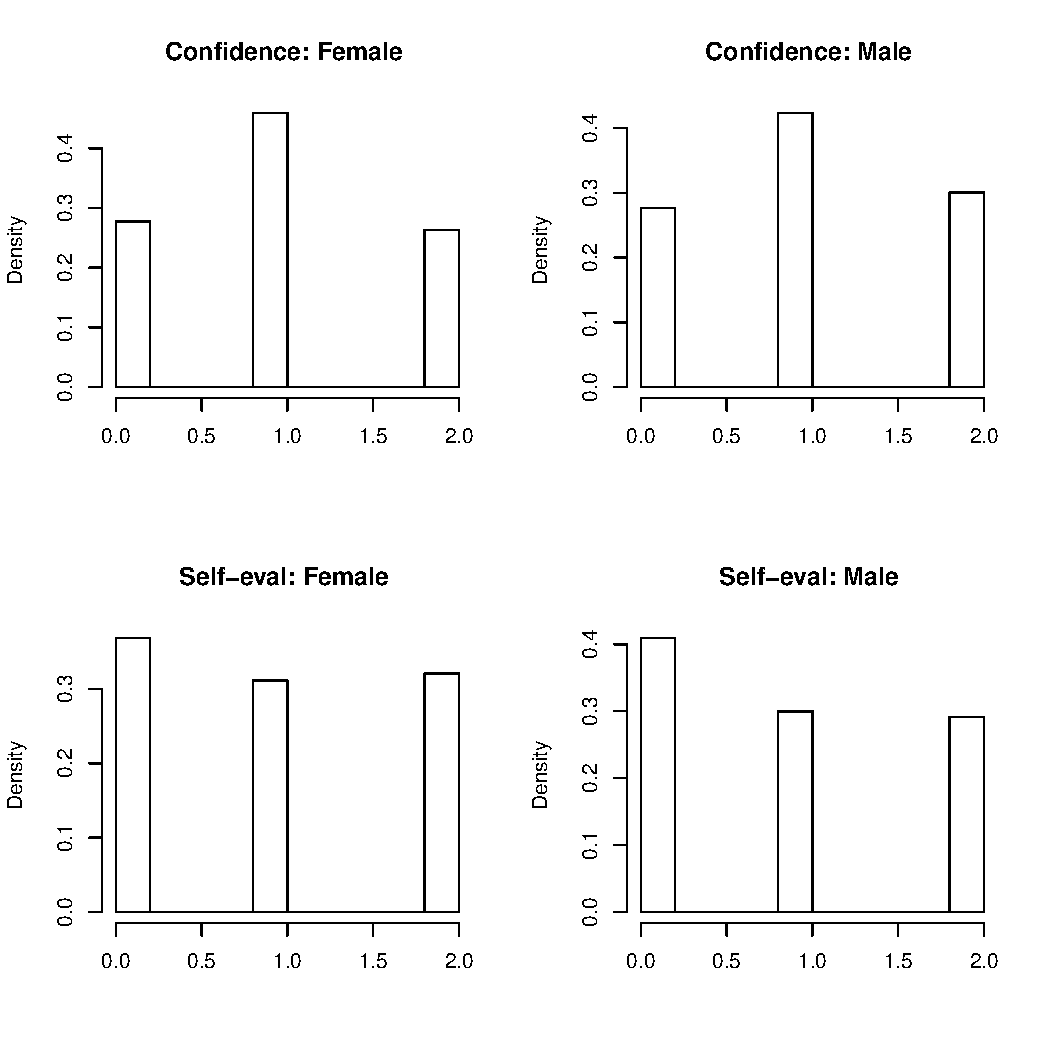
\includegraphics[width = 0.65 \textwidth]{comparison2.pdf}
\end{figure}
\noindent
Now consider the distribution of the different self evaluation levels \textit{conditional on different confidence levels}. Here too we note that the conditional distributions across male and female students are very similar. 


%\begin{minipage}{.3\textwidth}
% latex table generated in R 3.2.1 by xtable 1.8-2 package
% 
\begin{table}[H]\small
\centering
\caption{Males: Distribution of selfeval conditional on confidence}
\begin{tabular}{rrrr}
  \hline
 & Different & Close & Correct \\ 
  \hline
Low Conf & 0.66 & 0.24 & 0.10 \\ 
  Moderate Conf & 0.43 & 0.34 & 0.24 \\ 
  High Conf & 0.11 & 0.30 & 0.59 \\ 
   \hline
\end{tabular}
\end{table}
%\end{minipage}
%\begin{minipage}{.3\textwidth}
%\hspace{5em}
%\end{minipage}
%\begin{minipage}{.3\textwidth}
% latex table generated in R 3.2.1 by xtable 1.8-2 package
% 

\begin{table}[H]\small
\centering 
\caption{Females: Distribution of selfeval conditional on confidence}
\begin{tabular}{rrrr}
  \hline
 & Different & Close & Correct \\ 
  \hline
Low Conf & 0.63 & 0.24 & 0.13 \\ 
  Moderate Conf & 0.38 & 0.38 & 0.24 \\ 
  High Conf & 0.13 & 0.27 & 0.60 \\ 
   \hline
\end{tabular}
\end{table}
%\end{minipage}



\begin{figure}[H]
\centering
\caption{Histograms of self evaluation scores conditional on different confidence levels }
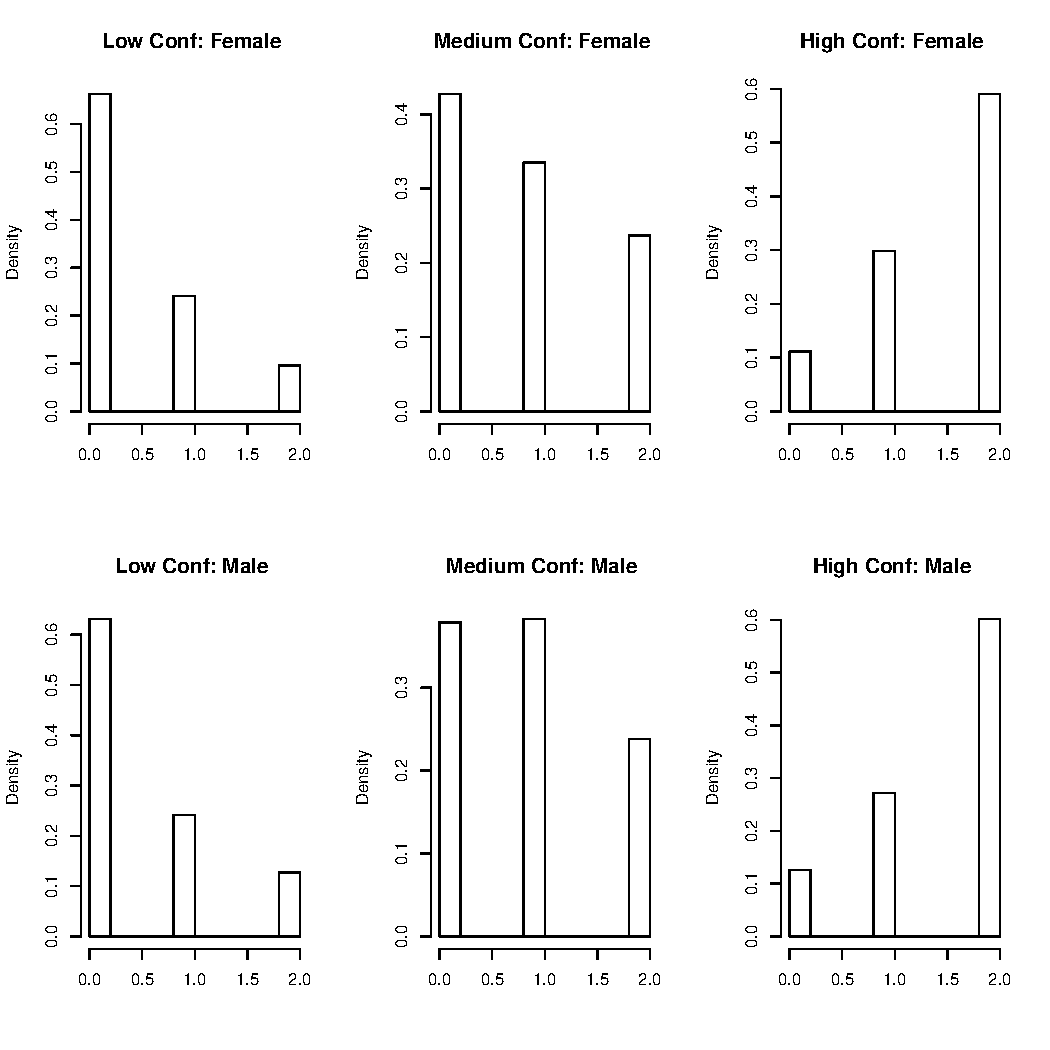
\includegraphics[width = 0.55 \textwidth]{comparison3.pdf}
\end{figure}
\noindent
The graphs and tables generated so far were from the Full Data. As a final visual summary, we use the Means Data --  consider the joint distribution of mean self evaluation and mean confidence for male and female students. These also appear to have a similar positive slope -- implying that the more confident a student is before submitting a response the more likely s/he is to self-report a ``correct" self evaluation, and that these rates are similar for both genders. 

\begin{figure}[H]
\caption{Joint distribution of mean self evaluation and mean confidence by gender }
\centering
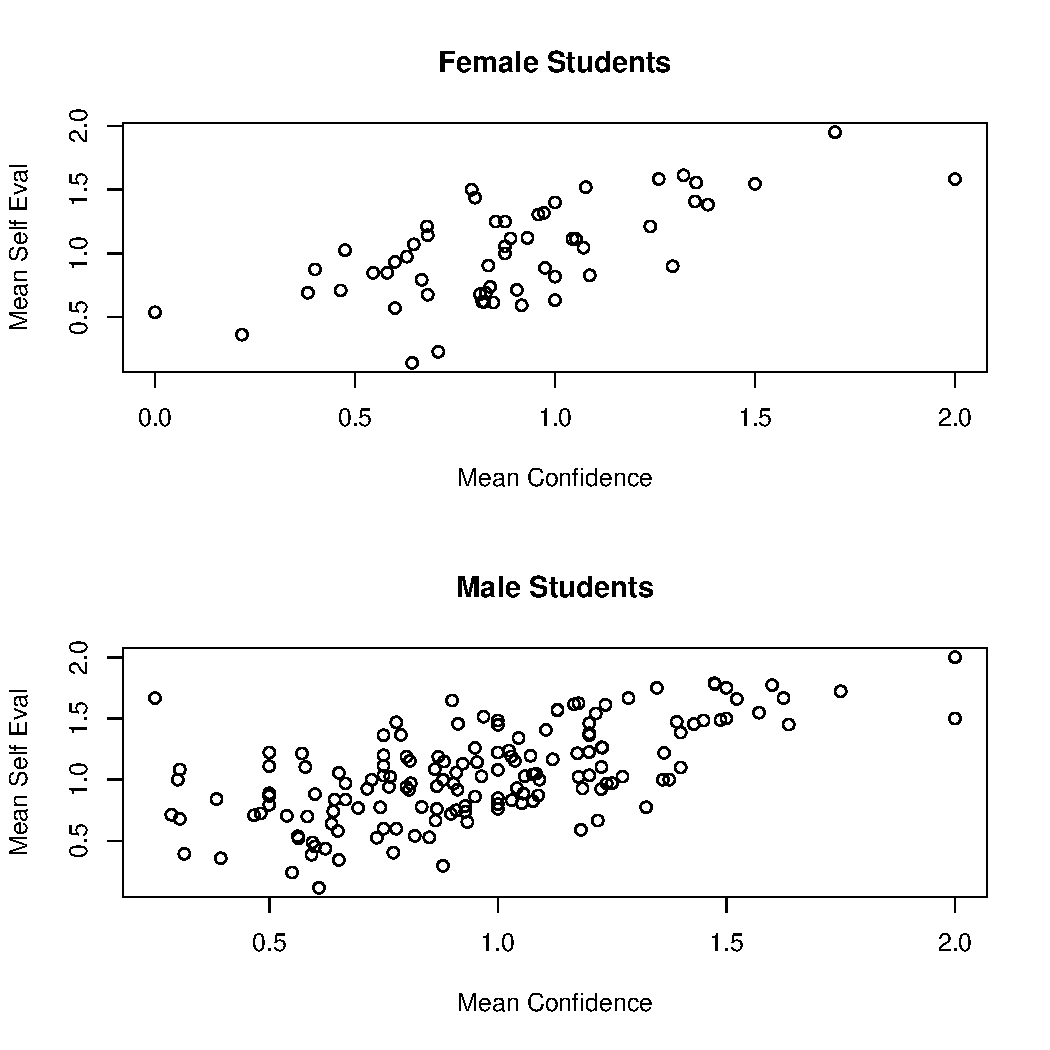
\includegraphics[width = 0.5 \textwidth]{comparison4.pdf}
\end{figure}



\subsection{Student Characteristics}
The composition of students in terms of ethnicity, proficiency levels and class terms is presented here to get a better idea of the study sample. Overall the distribution appears similar for both genders, except that there appears to be a slightly larger propertion of Male students in Term 12. 

\begin{figure}[H]
\centering
\caption{Student characteristics by gender}
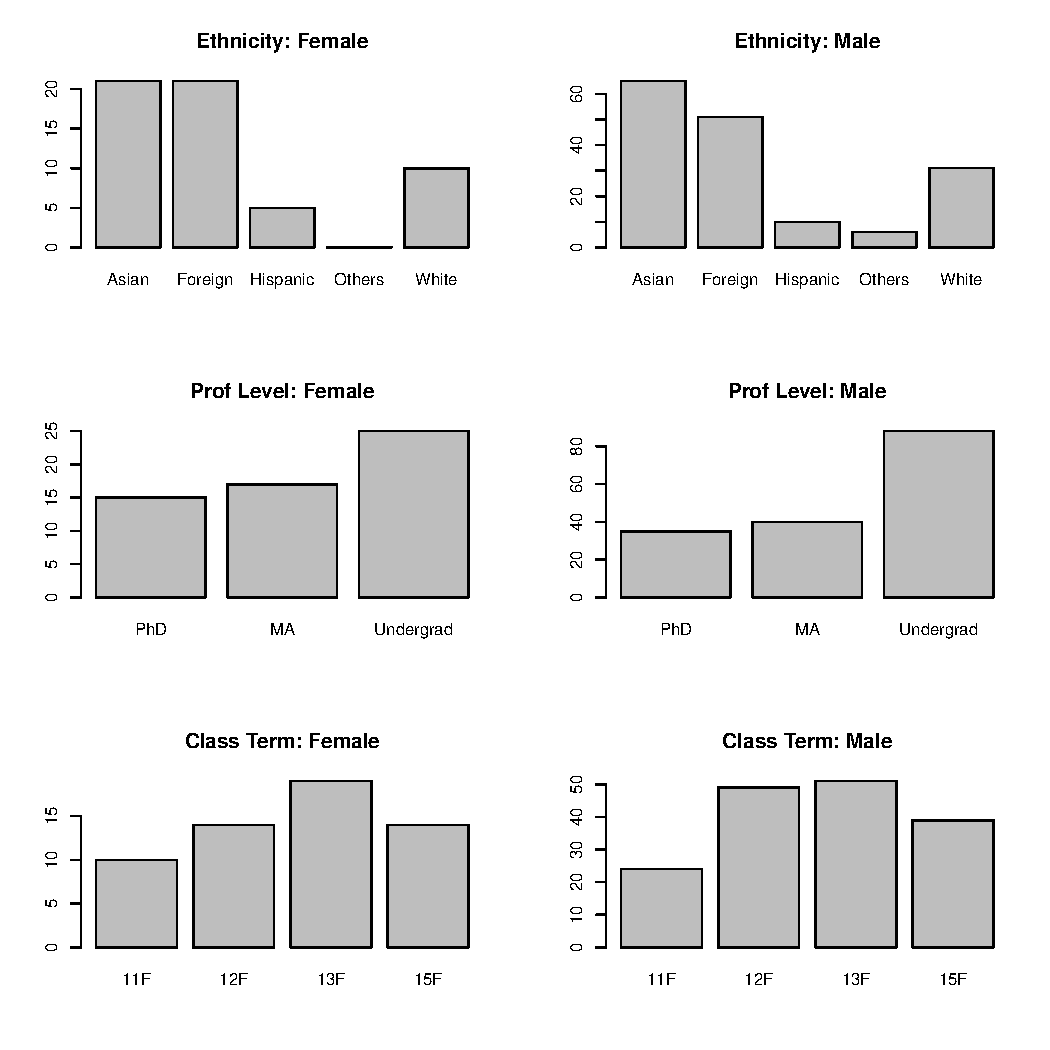
\includegraphics[width = 0.75 \textwidth]{comparison5.pdf}
\end{figure}




\section{Analysis 2: Regressions}
In this section, results from selected regressions are presented. 

\subsection{Set 1: Regressions using Means Data}
From regressions on the Means Data we get the following broad insights:
\begin{itemize}
\item[1.] Mean Self Evaluation is strongly and positively correlated with Mean Self Confidence -- implying that students are quite good at guessing how they will perform in the exercises (under the assumption that students' self evaluation is consistent with external evaluation). At this level of aggregation, there does not appear to be a significant impact of gender.
\item[2.] Mean confidence is strongly and positively correlated with being a graduate student. 
\item[3.] Number of questions answered is positively correlated with being a graduate student and \textit{negatively} correlated with mean confidence. This implies that the Full Data is biased towards students with lower confidence scores. (need to think this through -- discuss with Chris and team).
\end{itemize}
\subsubsection{Dependent Variable: Mean Self Eval}

\begin{table}[H]
\centering
% latex table generated in R 3.2.1 by xtable 1.8-2 package
% 
\begin{tabular}{rrrrr}
  \hline
 & Estimate & Std. Error & t value & Pr($>$$|$t$|$) \\ 
  \hline
(Intercept) & 0.4798 & 0.1984 & 2.42 & 0.0165 \\ 
  mean\_conf & \textbf{0.5873} & 0.0517 & 11.36 & 0.0000 \\ 
  female & -0.0420 & 0.0410 & -1.03 & 0.3062 \\ 
  age & -0.0112 & 0.0082 & -1.37 & 0.1724 \\ 
  phd & 0.0013 & 0.0632 & 0.02 & 0.9834 \\ 
  ma & 0.0807 & 0.0542 & 1.49 & 0.1378 \\ 
  asian & -0.0015 & 0.0502 & -0.03 & 0.9768 \\ 
  hispanic & -0.0777 & 0.0799 & -0.97 & 0.3321 \\ 
  foreign & 0.0577 & 0.0533 & 1.08 & 0.2808 \\ 
  term11 & 0.0739 & 0.0598 & 1.24 & 0.2183 \\ 
  term12 & \textbf{0.1680} & 0.0511 & 3.29 & 0.0012 \\ 
  term13 & 0.0783 & 0.0503 & 1.56 & 0.1209 \\ 
   \hline
\end{tabular}
\end{table}


\subsubsection{Dependent Variable: Number of Questions}


% latex table generated in R 3.2.1 by xtable 1.8-2 package
% Thu Aug  4 22:14:21 2016
\begin{table}[H]
\centering
\begin{tabular}{rrrrr}
  \hline
 & Estimate & Std. Error & t value & Pr($>$$|$t$|$) \\ 
  \hline
(Intercept) & 46.8669 & 6.6975 & 7.00 & 0.0000 \\ 
  mean\_conf & \textbf{-5.7358} & 1.7444 & -3.29 & 0.0012 \\ 
  female & 0.9821 & 1.3825 & 0.71 & 0.4783 \\ 
  age & -0.6308 & 0.2760 & -2.29 & 0.0234 \\ 
  phd & \textbf{7.4089} & 2.1326 & 3.47 & 0.0006 \\ 
  ma & \textbf{5.9852} & 1.8283 & 3.27 & 0.0013 \\ 
  asian & 0.4558 & 1.6959 & 0.27 & 0.7884 \\ 
  hispanic & 1.8219 & 2.6984 & 0.68 & 0.5004 \\ 
  foreign & -1.9891 & 1.7996 & -1.11 & 0.2703 \\ 
  term11 & -2.0703 & 2.0198 & -1.02 & 0.3066 \\ 
  term12 &\textbf{ 6.5779} & 1.7244 & 3.81 & 0.0002 \\ 
  term13 & -0.7567 & 1.6967 & -0.45 & 0.6561 \\ 
   \hline
\end{tabular}
\end{table}

\subsubsection{Dependent Variable: Mean Confidence}

\begin{table}[H]
\centering
% latex table generated in R 3.2.1 by xtable 1.8-2 package
% 
\begin{tabular}{rrrrr}
  \hline
 & Estimate & Std. Error & t value & Pr($>$$|$t$|$) \\ 
  \hline
(Intercept) & 1.3367 & 0.2545 & 5.25 & 0.0000 \\ 
  female &-0.0728 & 0.0558 & -1.31 & 0.1933 \\ 
  age & -0.0132 & 0.0112 & -1.19 & 0.2367 \\ 
  phd & \textbf{0.3444} & 0.0829 & 4.15 & 0.0000 \\ 
  ma & \textbf{0.2412} & 0.0721 & 3.34 & 0.0010 \\ 
  asian &-0.1432 & 0.0680 & -2.11 & 0.0364 \\ 
  hispanic & -0.1703 & 0.1087 & -1.57 & 0.1189 \\ 
  foreign &-0.1109 & 0.0725 & -1.53 & 0.1280 \\ 
  term11 & -0.0455 & 0.0818 & -0.56 & 0.5788 \\ 
  term12 & -0.0872& 0.0696 & -1.25 & 0.2120 \\ 
  term13 & 0.0605 & 0.0686 & 0.88 & 0.3791 \\ 
   \hline
\end{tabular}
\end{table}



\subsection{Set 2: Regressions using Full Data}

From regressions on the Full Data we get the following broad insights:
\begin{itemize}
\item[1.] Self Evaluation is again strongly and positively correlated with Confidence
\item[2.] Confidence is significantly affected by a number of factors. While being enrolled in a PhD or MA has a large  positive impact (as was the case with the Means Data), belonging to Hispanic, Asian or Foreign ethnicities has large negative impact. Age and gender (female) have smaller negative impacts.
\item[3.] Given the observation above, it may be worthwhile to study if  (like female students) dropout rates have also fallen for students of particular ethnicities since the introduction of ORCT. If our hypothesis is that the decrease in female dropouts is linked to confidence, then we should see similar patterns for say Asian and Hispanic students too.
\end{itemize}


\subsubsection{Dependent Variable: Self Evaluation}

\begin{table}[H]
\centering
% latex table generated in R 3.2.1 by xtable 1.8-2 package
% 
\begin{tabular}{rrrrr}
  \hline
 & Estimate & Std. Error & t value & Pr($>$$|$t$|$) \\ 
  \hline
(Intercept) & 0.5186 & 0.1103 & 4.70 & 0.0000 \\ 
  conf & \textbf{0.4997} & 0.0138 & 36.22 & 0.0000 \\ 
  female & -0.0374 & 0.0231 & -1.62 & 0.1062 \\ 
  age & -0.0070 & 0.0048 & -1.44 & 0.1492 \\ 
  phd & 0.0229 & 0.0355 & 0.64 & 0.5197 \\ 
  ma & 0.0403 & 0.0310 & 1.30 & 0.1932 \\ 
  asian & -0.0197 & 0.0287 & -0.69 & 0.4931 \\ 
  hispanic & -0.0924 & 0.0437 & -2.12 & 0.0344 \\ 
  foreign & 0.0794 & 0.0308 & 2.58 & 0.0100 \\ 
  term11 & -0.0040 & 0.0364 & -0.11 & 0.9116 \\ 
  term12 &\textbf{ 0.1262} & 0.0258 & 4.89 & 0.0000 \\ 
  term13 & 0.0082 & 0.0291 & 0.28 & 0.7775 \\ 
   \hline
\end{tabular}
\end{table}

\subsubsection{Dependent Variable: Confidence}


\begin{table}[H]
\centering
% latex table generated in R 3.2.1 by xtable 1.8-2 package
% 
\begin{tabular}{rrrrr}
  \hline
 & Estimate & Std. Error & t value & Pr($>$$|$t$|$) \\ 
  \hline
(Intercept) & 1.5792 & 0.0946 & 16.70 & 0.0000 \\ 
  female &\textbf{ -0.0595} & 0.0202 & -2.95 & 0.0032 \\ 
  age & \textbf{-0.0238} & 0.0042 & -5.68 & 0.0000 \\ 
  phd & \textbf{0.3431} & 0.0311 & 11.03 & 0.0000 \\ 
  ma & \textbf{0.2306} & 0.0268 & 8.60 & 0.0000 \\ 
  asian & \textbf{-0.1486} & 0.0253 & -5.88 & 0.0000 \\ 
  hispanic & \textbf{-0.2120} & 0.0383 & -5.54 & 0.0000 \\ 
  foreign &\textbf{ -0.1257} & 0.0270 & -4.66 & 0.0000 \\ 
  term11 & -0.0593 & 0.0307 & -1.93 & 0.0533 \\ 
  term12 &\textbf{ -0.0855} & 0.0241 & -3.54 & 0.0004 \\ 
  term13 & 0.0268 & 0.0253 & 1.06 & 0.2890 \\ 
   \hline
\end{tabular}
\end{table}

\section{Analysis 3: Confidence Trajectories}
For each student we know how many questions s/he attempted and the corresponding self-reported confidence and submit times. These can be used to track how a given student's mean confidence evolves over time. To visualize this, the mean confidence for each student after $n$ questions is calculated and then plotted against the question index. A few sample trajectories are presented next. These graphs are generated using only the student response data. Note that the x-axis limits for these are different since different students submitted different number of responses. \\\\
At this point we are still trying to think of a statistically valid way to use these trajectories, for now they provide us with some visual cue on a student's progress/evolution over the course of the exercises. 
\begin{figure}[H]
\centering
\caption{Sample mean confidence trajectories -- each figure corresponds to a unique student}
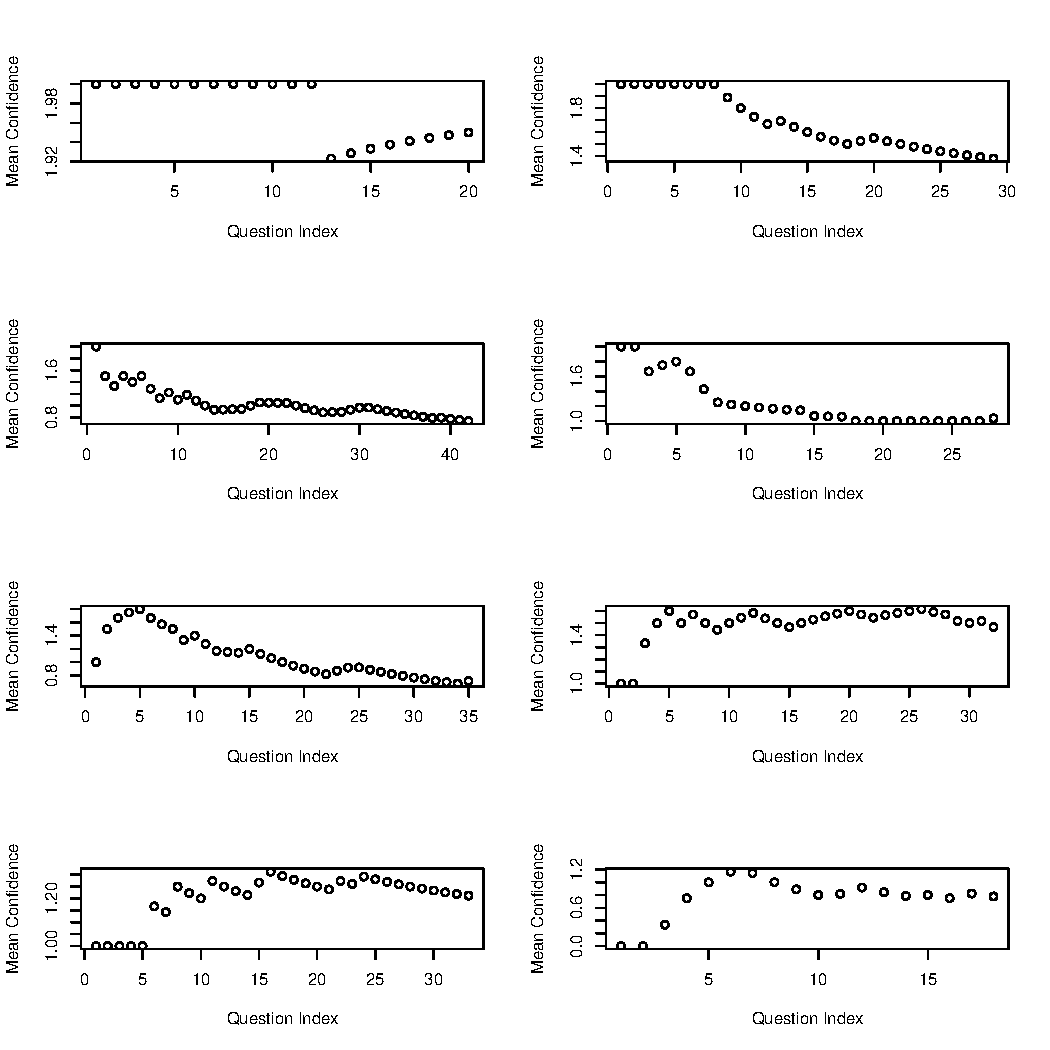
\includegraphics[width =  \textwidth]{trajectories1.pdf}
\end{figure}




\end{document}

\section{Next Steps and Methodological Questions}
A number of next steps and open questions arise 


\begin{itemize}

\item Next Step: When we have Week 1 data -- compare those who dropped out with those who completed the course

\item Next Step: At this point didn't use many student characteristics (like ) because of large number of missing values, incorporate these variables after imputations or finding subsets with no missing values

\item Next Step: Employ matching techniques 

\item What kind of conditions can we impose on the full data to address the issue of variation in representation. Currently its an unbalanced panel

\item The Mean Data does not imply , but the Full Data does -- however it shows stronger negative effects for Asian, Hispanic and Foreign students

\item What is a smart and statistically valid way to compare trajectories? 

\end{itemize}



